\documentclass[conference]{IEEEtran}
\usepackage{graphicx}
\graphicspath{{../figures/}}
\usepackage{cite}
\usepackage{amsmath}
\usepackage{url}
\usepackage{balance}
\usepackage[hidelinks]{hyperref}
\usepackage{booktabs}
\usepackage{listings}
\lstset{
  basicstyle=\footnotesize\ttfamily,
  numbers=left,
  numberstyle=\tiny,
  numbersep=5pt,
  frame=single,
  breaklines=true,
  captionpos=b,
  xleftmargin=2em,
  framexleftmargin=1.5em
}



\begin{document}

\title{Coordinated Graph and Matrix Views for TLA+ State Space Comprehension: A Design Study}

\author{
\IEEEauthorblockN{Anonymous Author(s)}
\IEEEauthorblockA{Anonymous Affiliation\\
Anonymous City, Anonymous Country\\
anonymous@email.com}
}

\maketitle

\begin{abstract}
Mission-critical systems have to comply with rigorous formal standards, yet the state spaces produced by model checkers like TLC are difficult for engineers to comprehend. Standard node-link visualisations degenerate into illegible tangles beyond a few dozen states. We present a multi-view visualisation tool for TLA+ state spaces that combines a clustered force-directed graph, an adjacency matrix with cluster-based ordering, and a coordinated split view with bidirectional brushing-and-linking. The tool groups states by shared variable values, enabling engineers to understand state structure, verify transitions, and trace execution paths. We describe our design process, including task analysis, data characterisation, and design rationale, and demonstrate the tool on two TLA+ specifications of increasing complexity.
\end{abstract}

\begin{IEEEkeywords}
formal methods, TLA+, visualisation, state machine, adjacency matrix, coordinated views, design study, model checking
\end{IEEEkeywords}

\section{Introduction}

Formal system specification provides significant advantages for mission-critical systems engineering. Mission-critical systems have to comply with rigorous standards, such as DO-178C for airborne software and ISO~26262 for automotive functional safety, that rely heavily on mathematical formalisms to establish correctness. Among formal specification languages, TLA+ (Temporal Logic of Actions)~\cite{lamport2003specifying, lamport2009pluscal} has emerged as one of the most widely adopted in industry. Amazon Web Services uses TLA+ to verify the correctness of complex distributed systems including DynamoDB, S3, and EBS~\cite{newcombe2015amazon}, while Microsoft has applied TLA+ to safety-critical fault-tolerant middleware~\cite{resch2017tla}. The TLC model checker~\cite{yuan1999model} enables engineers to exhaustively enumerate all reachable states and transitions for a given specification.

However, these specifications require deep expertise in temporal logic. For many systems engineers, TLA+ specifications and models are very hard to read and review, limiting usability. We want to aid these engineers by applying visualisation techniques to translate TLA+ state spaces into intuitive visual representations, such as state machine diagrams~\cite{harel1987statecharts, harel1988visual}. However, the state spaces produced by model checking are inherently difficult to comprehend: even for moderately complex specifications, the number of reachable states grows combinatorially with the number of variables and their domains~\cite{liu2005model}. Standard force-directed layouts degenerate into illegible ``hairball'' diagrams beyond a few dozen states, a well-documented scalability limitation~\cite{herman2000graph}.

Research in information visualisation has established that different visual representations have complementary strengths. Ghoniem et al.~\cite{ghoniem2004comparison} demonstrated that adjacency matrices outperform node-link diagrams for dense graphs on tasks such as finding connections, while node-link diagrams remain superior for path-following tasks. Henry and Fekete~\cite{henry2006matrixexplorer} showed that combining both representations in a coordinated dual-representation system enables users to leverage the strengths of each. The TensorFlow Graph Visualizer~\cite{wongsuphasawat2018tensorflow} demonstrated that hierarchical clustering, semantic grouping, and interactive detail-on-demand can make computational graphs with thousands of nodes navigable.

Drawing on these insights, we present a design study~\cite{sedlmair2012design} of a multi-view visualisation tool for TLA+ state spaces. We make the following contributions:

\begin{itemize}
\item A \textbf{task analysis} for TLA+ state space visualisation, identifying four key tasks engineers need to perform.
\item A \textbf{clustered force-directed graph view} that groups states by shared variable values, with convex hull cluster boundaries, colour-coded cluster membership, and interactive detail-on-demand.
\item An \textbf{adjacency matrix view} with cluster-based ordering that reveals connectivity patterns and cluster structure at higher information density than node-link diagrams.
\item A \textbf{coordinated split view} with bidirectional brushing-and-linking: hovering a state in either view highlights the corresponding state and its connections in the other view.
\item \textbf{Usage scenarios} on two TLA+ specifications of increasing complexity, demonstrating how the multi-view approach supports each identified task.
\end{itemize}

\section{Background and Related Work}

\subsection{TLA+ and Model Checking}

TLA+ is a formal specification language created by Leslie Lamport for specifying and reasoning about concurrent and distributed systems~\cite{lamport2003specifying}. TLA+ specifications describe a system as a state machine: an initial state predicate defines the set of possible starting states, and a next-state relation defines how the system can transition from one state to another. Each state is a complete assignment of values to all specification variables, and each transition is triggered by an action.

The TLC model checker~\cite{yuan1999model} is the primary verification tool for TLA+ specifications. Given a specification and model constraints, TLC exhaustively enumerates all reachable states and transitions using breadth-first search, producing a complete state graph $G = (V, E)$ where each vertex $v \in V$ represents a distinct reachable state and each directed edge $(u, v) \in E$ represents a transition. A fundamental challenge is the state explosion problem: the number of reachable states grows combinatorially with the number of specification variables and their domains.

\subsection{Related Work}

Visualisation of formal specifications has received attention across multiple communities. Harel's Statecharts~\cite{harel1987statecharts} introduced a visual formalism for hierarchical state machines that has influenced specification languages and their visualisation tools. For TLA+ specifically, the TLA+ Toolbox provides the TLC model checker with textual output but does not include graphical visualisation of the state space. Other formal methods tools provide visualisation capabilities for their respective languages: the Alloy Analyser~\cite{jackson2012alloy} visualises instances as node-link diagrams, ProB~\cite{leuschel2008prob} provides a graphical state space viewer for the B-method~\cite{abrial1996bbook}, and UPPAAL~\cite{behrmann2004uppaal} provides a graphical editor for timed automata. Across these tools, a common limitation is the reliance on standard node-link diagrams, which inherently limits scalability.

In graph visualisation, clustered graph drawing~\cite{eades1996hierarchical} and hierarchical layouts~\cite{sugiyama1981hierarchical} address some scalability problems. Adjacency matrices provide a fundamentally different representation that avoids edge crossings entirely~\cite{bertin1983semiology, behrisch2016reordering}. The principle of coordinated multiple views (CMV)~\cite{roberts2007cmv} is well-established in information visualisation, with Shneiderman's visual information seeking mantra~\cite{shneiderman1996eyes} providing the theoretical basis. Our coordinated split view implements bidirectional brushing-and-linking between the graph and matrix views, following the design guidelines of Baldonado et al.~\cite{baldonado2000guidelines} and the tight coupling approach of North and Shneiderman~\cite{north2000snap}.

\section{Design Process}

Our tool was developed through an iterative design process informed by our experience in TLA+ specifications in industry projects. We followed the design study methodology described by Sedlmair et al.~\cite{sedlmair2012design}. Following Munzner's nested model~\cite{munzner2009nested}, our task analysis addresses the domain level, our data model addresses the abstraction level, and our view designs address the encoding level.

\subsection{Task Analysis}

From our experience deploying TLA+ specifications in industry projects, we identified four key tasks, ordered from high-level overview to detailed inspection following Shneiderman's visual information seeking mantra~\cite{shneiderman1996eyes}:

\begin{itemize}
\item \textbf{T1. Overview.} Understand the high-level structure of the state space; how many states exist, how they cluster, and the overall connectivity pattern.
\item \textbf{T2. Cluster identification.} Recognise groups of states that share common variable values, which often correspond to meaningful system modes or phases.
\item \textbf{T3. Transition inspection.} Examine specific transitions between states to verify that the specification correctly defines how the system moves between states.
\item \textbf{T4. Path tracing.} Follow sequences of transitions to understand system behaviour under specific scenarios, directly supporting debugging of TLA+ specifications.
\end{itemize}

\subsection{Data Characterisation}

The TLC model checker produces a directed graph $G = (V, E)$ where each vertex $v \in V$ is a state and each directed edge $(u, v) \in E$ is a transition. Each state is characterised by a unique identifier, a label describing its variable assignments, and a cluster identifier derived from the value of one or more grouping variables. We identified four data characteristics specific to TLA+ state spaces: \textbf{C1.}~Variable-based clustering (states naturally group by shared variable values); \textbf{C2.}~Dense inter-cluster connectivity (actions that change the grouping variable create transitions between clusters); \textbf{C3.}~Action-labelled transitions; and \textbf{C4.}~Moderate scale (the most common use case involves specifications with 10--200 states).

\subsection{Design Challenges and Rationale}

We identified three design challenges: \textbf{D1.}~Mismatch between topology and semantics (the spatial layout of a force-directed graph does not necessarily reflect the semantic structure), corresponding to the challenge identified by Wongsuphasawat et al.~\cite{wongsuphasawat2018tensorflow} for TensorFlow graphs; \textbf{D2.}~Visual clutter from dense connectivity (C2 causes severe visual clutter in node-link diagrams); and \textbf{D3.}~Task diversity (the four tasks require different visual representations---no single view optimally supports all four).

We explored three design approaches and selected \textbf{Approach~C: Combination of graph and matrix views}. This approach provides both views simultaneously in a coordinated split view, leveraging the complementary strengths of each representation to address all three design challenges. The clustered graph view addresses D1 by using cluster forces to spatially group semantically related states. The matrix view addresses D2 by providing a clutter-free representation. The coordinated split view addresses D3 by enabling engineers to use the most appropriate representation for each task while maintaining context through bidirectional linking, aligning with the design principles established by Henry and Fekete~\cite{henry2006matrixexplorer}.

\section{Multi-View Visualisation Tool}

The tool is implemented as a web application using HTML, CSS, and JavaScript, with D3.js~\cite{bostock2011d3} providing the visualisation primitives. It consists of three views: clustered graph view, adjacency matrix view, and coordinated split view. Each view can be used independently or in combination through the split view, which embeds the graph and matrix views as iframes and coordinates their interactions through the browser's \texttt{postMessage} API.

\subsection{Clustered Force-Directed Graph View}

The graph view renders the state space as a clustered force-directed layout. The layout uses D3's force simulation with five forces: centering, charge repulsion, collision detection, cluster attraction (pulling nodes toward the centroid of their cluster), and link constraint. Nodes are rendered as circles coloured by cluster membership. Edges between nodes are rendered as paths; for pairs of nodes with bidirectional transitions, the default view shows a single slightly thicker line to reduce clutter. Convex hulls are drawn around clusters with two or more members using a semi-transparent fill of the cluster colour.

\textbf{Interaction.} Hovering over a node triggers a progressive disclosure interaction: the selected node and its immediate neighbours remain at full opacity, while all other nodes fade to 20\% opacity. Connected edges turn red and display directional arrowheads; for bidirectional pairs, the single default line splits into two curved edges with arrowheads showing each direction. A tooltip displays the state label, cluster identifier, and in/out degree.

\textbf{Cluster-level aggregation.} For clusters with two or more members, a centroid circle is drawn at the cluster centre. Aggregate cluster-level edges connect clusters with curved arcs whose thickness encodes the number of individual transitions between those clusters. Clicking a cluster-level edge reveals the individual node-to-node transitions, enabling drill-down from overview to detail following Shneiderman's visual information seeking mantra~\cite{shneiderman1996eyes}.

\subsection{Adjacency Matrix View}

The matrix view renders the state-transition graph as an adjacency matrix. The matrix is ordered by cluster membership (default), grouping states belonging to the same cluster together along the diagonal. A filled (black) cell at position $(i,j)$ indicates a transition from state $i$ to state $j$. Cells within the same cluster are lightly shaded with the cluster colour at 40\% opacity, making cluster boundaries immediately visible as coloured blocks along the diagonal. Hovering over a row or column label highlights that state's entire row and column, with connected cells outlined in red. The matrix supports reordering by cluster (default) or by node identifier.

\subsection{Coordinated Split View}

The split view displays the graph and matrix views side by side in a 3:2 width ratio. Both views are embedded as iframes, with a shared toolbar for file upload and clear controls. The bidirectional highlighting is implemented through the \texttt{postMessage} API: hovering a state in one view sends a \texttt{highlight} message that the parent window forwards to the other view. This coordination supports a cross-referencing workflow: an engineer can identify an interesting cluster in the matrix and then hover over a state in that block to immediately locate it spatially in the graph view, and vice versa.

\section{Usage Scenarios}

We demonstrate our tool on two TLA+ specifications drawn from the formal methods literature, following the design study methodology~\cite{sedlmair2012design}.

\subsection{HourClock: Simple Cyclic Behaviour}


The HourClock specification~\cite{lamport2003specifying} is a canonical TLA+ example: a single variable \texttt{hr} cycles through values 1 to 12 governed by a single action HCnxt, producing 12 states in a single cluster. Fig.~\ref{fig:hourclock_spec} shows the TLA+ specification.



\begin{figure}[t]
\begin{lstlisting}[language={},morekeywords={MODULE,EXTENDS,VARIABLE,IF,THEN,ELSE,THEOREM}]
---- MODULE HourClock ----
EXTENDS Naturals
VARIABLE hr
HCini == hr \in (1 .. 12)
HCnxt == hr' = IF hr # 12
                THEN hr + 1
                ELSE 1

HC == HCini /\ [][HCnxt]_hr
---------------------------
THEOREM HC => []HCini
===========================
\end{lstlisting}
\vspace{-0.5em}
\caption{The HourClock TLA+ specification~\cite{lamport2003specifying}. The variable \texttt{hr} ranges from 1 to 12, and the action \texttt{HCnxt} increments it cyclically.}
\label{fig:hourclock_spec}
\end{figure}

\begin{figure}[t]
\centering
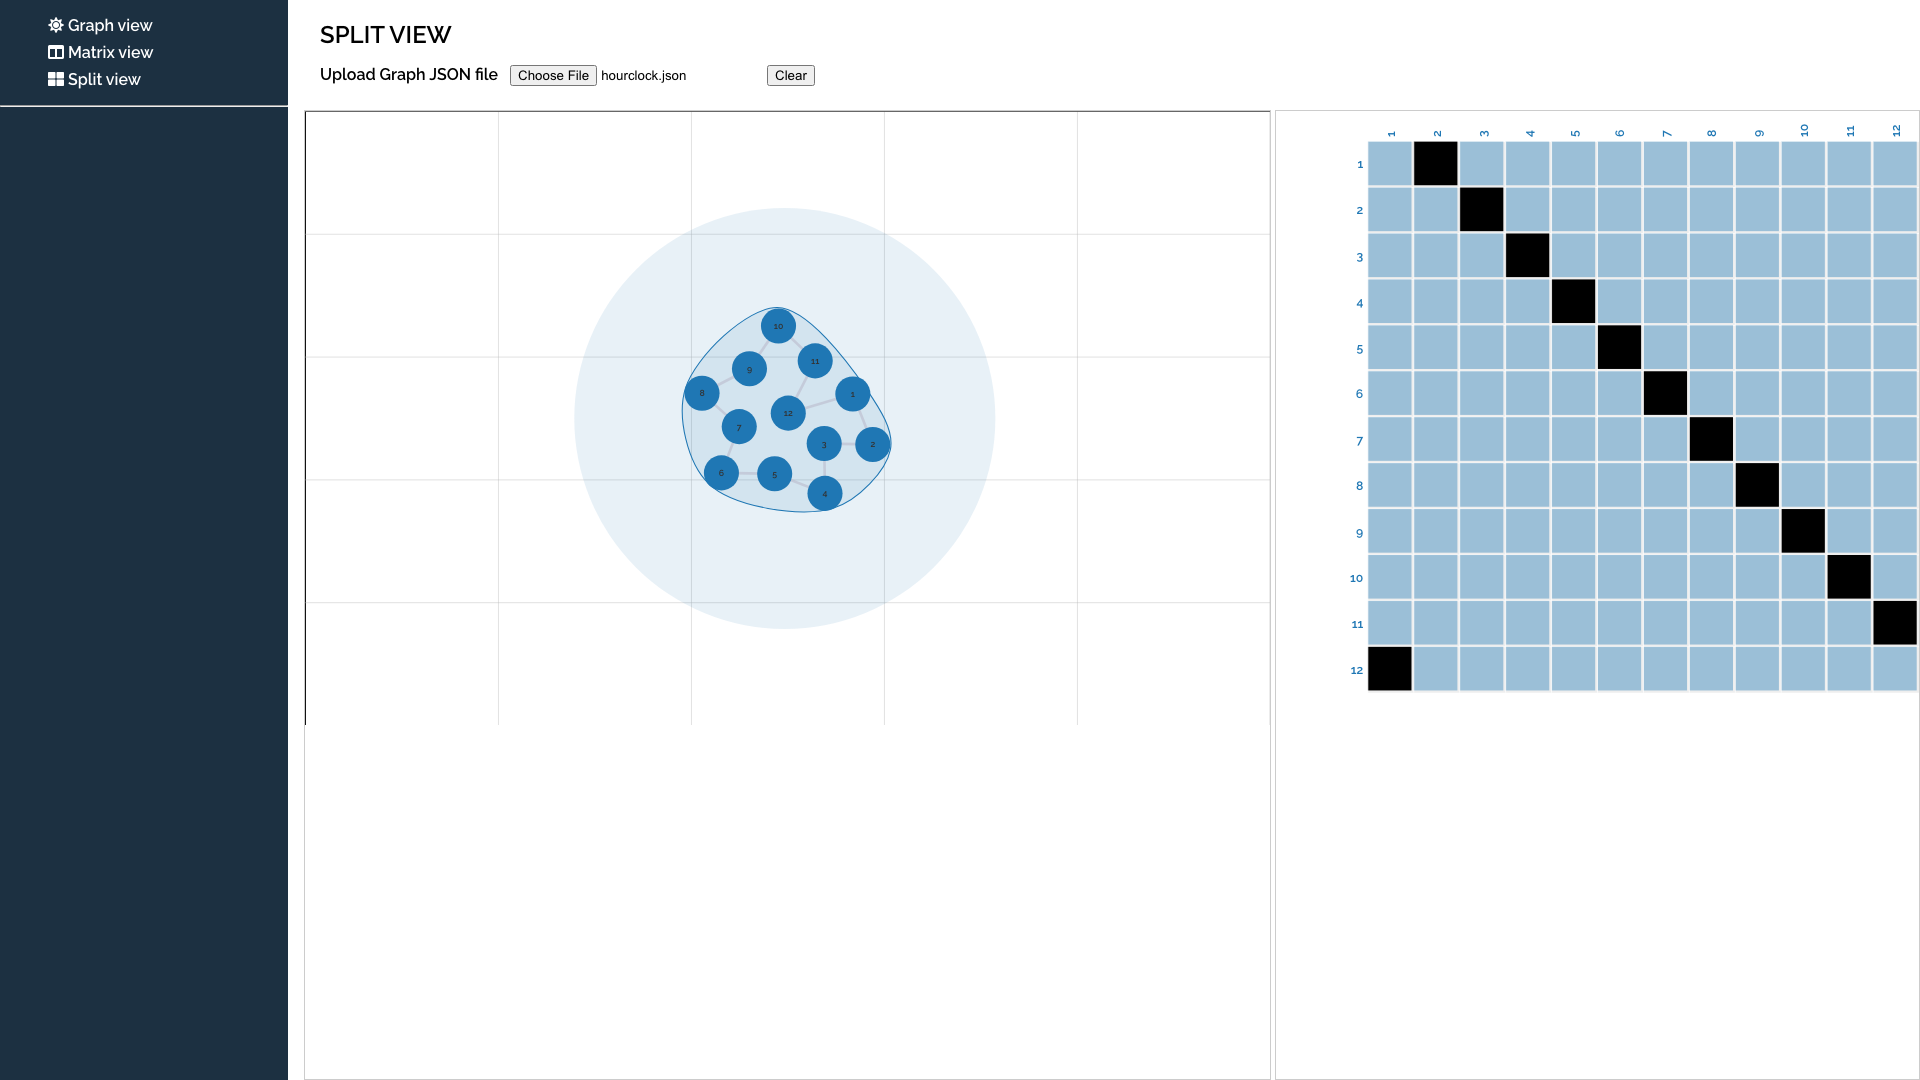
\includegraphics[width=\columnwidth]{figures/hourclock_split.png}
\caption{The coordinated split view for the HourClock specification. Left: 12 nodes in a single cluster arranged by force-directed layout. Right: adjacency matrix showing the cyclic pattern as a diagonal band one step above the main diagonal.}
\label{fig:hourclock}
\end{figure}


\begin{figure*}[!ht]
\centering
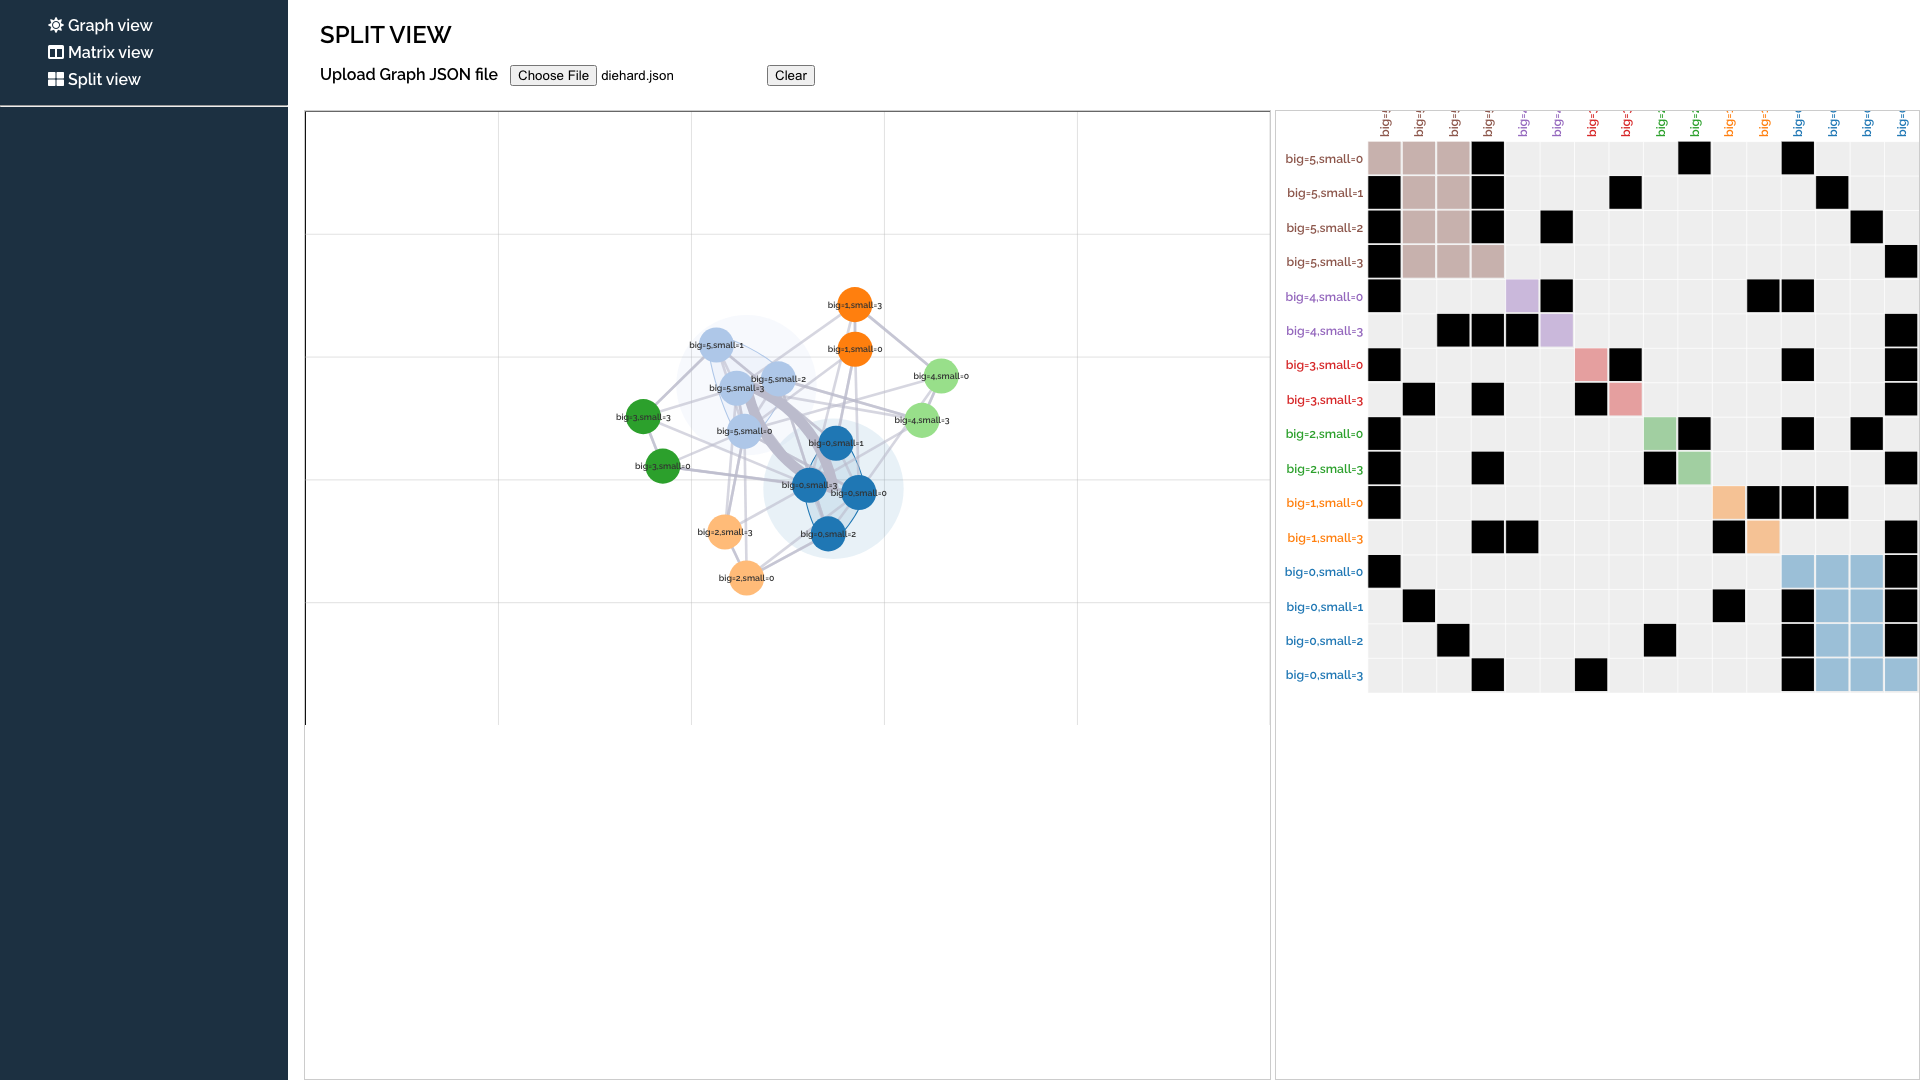
\includegraphics[width=\textwidth]{figures/diehard_split.png}
\caption{The coordinated split view showing the Die Hard water jugs specification (16 states, 58 transitions). Left: clustered force-directed graph with six clusters (one per \texttt{big}-jug value), colour-coded by cluster membership, with convex hulls delineating cluster boundaries and aggregate cluster-level edges whose thickness encodes transition count. Right: adjacency matrix ordered by cluster membership, with filled cells indicating transitions and coloured diagonal blocks marking cluster boundaries. Hovering a node in either view highlights connected edges and states in both views.}
\label{fig:splitview}
\end{figure*}

Fig.~\ref{fig:hourclock} illustrates a key insight about when each representation is most valuable. In the graph view (left), the 12 nodes are enclosed in one convex hull and arranged roughly in a circle by the force simulation---but the exact ordering around the ring depends on simulation convergence and is not guaranteed to reflect the logical 1--12 sequence. Confirming the cyclic ordering requires manually tracing each edge, a task that scales poorly even for this simple specification.

The matrix view (right) reveals the specification's structure unambiguously. The pattern is distinctive: a diagonal band of filled cells exactly one step above the main diagonal, plus a single isolated cell at position $(12, 1)$ for the wrap-around. This pattern is immediately recognisable as a deterministic cycle---every state has exactly one outgoing and one incoming transition, and no state is a dead end. An engineer can verify in seconds that the specification is deterministic, complete, and correctly cyclic. No edge tracing is required. This finding directly aligns with Ghoniem et al.~\cite{ghoniem2004comparison}: for specifications where precise connectivity assessment matters, the matrix is not merely comparable to the graph---it is strictly superior.

The coordinated view adds confirmation for T3: hovering \texttt{hr=6} in the graph immediately highlights row~6 and column~6 in the matrix, confirming one incoming transition (from \texttt{hr=5}) and one outgoing (to \texttt{hr=7}). For this regular specification the coordination is not essential---the matrix alone suffices---but it demonstrates the interaction protocol that becomes critical for the complex, multi-cluster case below.




\subsection{Die Hard Water Jugs: Clustering and Dense Transitions}


The specification models two jugs (5 and 3 gallons) with six actions (\texttt{FillBig}, \texttt{FillSmall}, \texttt{EmptyBig}, \texttt{EmptySmall}, \texttt{BigToSmall}, \texttt{SmallToBig}). States are grouped by the value of \texttt{big} into six clusters (\texttt{big=0} through \texttt{big=5}). With an average of 3.6 outgoing transitions per state, a flat node-link layout produces an illegible tangle with no discernible structure.

In Fig.~\ref{fig:splitview} (left), the \textbf{clustered graph view (T1, T2)} makes cluster structure immediately legible. Each cluster is enclosed in a colour-coded convex hull; the two largest clusters (\texttt{big=0} and \texttt{big=5}, each with four states) appear at opposite ends of the variable's range. The arc connecting them is among the thickest, correctly encoding that \texttt{FillBig} from any \texttt{big=0} state reaches \texttt{big=5} directly---the single most common transition type. This arc thickness encodes a structural insight that is invisible in a flat layout. Within clusters, nodes representing states with \texttt{big=1} or \texttt{big=2} are small two-state clusters, reflecting the constrained interactions possible at those jug levels. The spatial grouping allows an engineer to immediately identify which value of \texttt{big} represents the goal (\texttt{big=4}) and which clusters are likely predecessors, before inspecting any individual transition.



In Fig.~\ref{fig:splitview} (right), the \textbf{matrix view (T2, T3)} reveals a rich block structure invisible in the graph. Intra-cluster transitions appear as dense coloured blocks along the diagonal---clearly visible for \texttt{big=5} (top-left, a dense $4 \times 4$ block) and \texttt{big=0} (bottom-right). Off-diagonal filled cells show inter-cluster transitions; their asymmetric distribution confirms the directed nature of the graph. Two structural properties are immediately readable without hovering: boundary states where one or both jugs are completely full or empty have visibly fewer filled cells per row (fewer enabled actions); and no row is entirely empty (every state has at least one successor). These properties are impossible to verify at a glance in the graph view.



The \textbf{coordinated view (T3, T4)} enables path tracing toward the goal state \texttt{big=4,small=0}. Hovering this state in the graph highlights its column in the matrix (predecessor states) and row (successor states). Stepping backward through predecessors---re-hovering each to reveal its own incoming transitions---traces the solution path incrementally. At each step the graph provides spatial context (which cluster each predecessor belongs to) while the matrix provides precise connectivity (exactly which states feed into it and via which actions shown in the cell tooltip). Neither view alone supports this workflow: the graph lacks the precision for step-by-step verification, and the matrix lacks the spatial orientation to situate each predecessor in the broader state space.

\section{Discussion and Conclusion}

Our usage scenarios confirm three findings from the visualisation literature. First, graph and matrix representations have complementary strengths~\cite{ghoniem2004comparison, henry2006matrixexplorer}: the graph supports overview and cluster identification (T1, T2), while the matrix excels at transition inspection and structural verification (T3). The HourClock scenario demonstrates the matrix can be strictly superior for regular specifications; the Die Hard scenario shows neither view alone is sufficient for complex ones. Second, variable-based clustering is highly effective for TLA+ state spaces, where domain knowledge provides a semantically meaningful criterion more informative than topological community detection, directly analogous to namespace-based grouping for TensorFlow graphs~\cite{wongsuphasawat2018tensorflow}. Third, bidirectional brushing-and-linking proved essential for path tracing: the Die Hard scenario shows that alternating between spatial orientation (graph) and precise connectivity (matrix) enables step-by-step counterexample analysis that neither view supports alone, consistent with coordinated multiple views principles~\cite{baldonado2000guidelines, roberts2007cmv}.

Our tool targets TLA+ specifications with tens to low hundreds of states, the most common range for visual exploration. The clustered graph view performs well up to approximately 50 states; beyond this, inter-cluster edge density causes increasing clutter even with clustering. The adjacency matrix scales better, as the grid layout eliminates edge crossings regardless of graph density, but cell size and label readability degrade beyond approximately 100 states as the matrix grows quadratically ($n \times n$ cells for $n$ states). The coordinated view's effective ceiling is therefore bounded by whichever individual view degrades first for the task at hand. Scaling beyond these limits demands abstraction techniques such as hierarchical clustering with collapsible sub-clusters, but any visual abstraction risks hiding counterexamples or making unreachable paths appear connected, raising the question of whether ``visual soundness'' can be defined analogously to abstraction soundness in model checking, providing formal guarantees about when a simplified visualisation faithfully represents the underlying state space.

We have not yet conducted a formal user evaluation; the usage scenarios are based on our own expert analysis. A rigorous evaluation following two complementary tracks, qualitative feedback from engineers working with TLA+ in industry and a controlled user study comparing task performance across views, is our highest priority for future work. Additional future directions include direct integration with the TLC model checker to streamline the workflow, hierarchical edge bundling~\cite{holten2006hierarchical} to reduce visual clutter for dense cluster pairs, and bidirectional editing that propagates changes from the visualisation back to the TLA+ source.

Our tool addresses a practical need in the formal methods community: as TLA+ adoption grows in industry~\cite{newcombe2015amazon, resch2017tla}, engineers who are not formal methods experts need visual tools to comprehend the state spaces produced by model checking. By adapting techniques from the information visualisation literature to the specific structure of TLA+ state spaces, our tool makes formal specifications more accessible and supports the verification workflow on which mission-critical systems engineering depends.

\balance
\bibliographystyle{IEEEtran}
\bibliography{references}

\end{document}
